\subsection{Cryptanalyse par programmation dynamique}
\label{dyn}

Le code de Merkle-Hellman est un cas particulier du problème du sac à dos avec des objets qui auraient une valeur égale à leur masse. Il existe plusieurs algorithmes classiques permettant de trouver une solution à ce problème par force brute, notamment celui s'appuyant sur la programmation dynamique.

On peut donc voir le problème sous divers points de vue : 

\paragraph{} Un voleur se trouve dans une pièce où se trouvent 4 objets de masse $T = \{3, 2, 6, 4\}$. 
Quels objets doit-il choisir pour remplir exactement un sac de 7 kg ?
Dans le cadre de la cryptanalyse, l'ensemble ordonné $T$ constitue la clé 
publique, ici de taille 4, et la capacité maximale du sac $y = 7$, le bloc chiffré.

\paragraph{} On utilisera un tableau de 5 lignes et 8 colonnes qu'on complètera avec des 1 si une solution existe pour le sous-problème correspondant, des 0 sinon. La case rouge de la figure \ref{dyn1} indique donc que le problème
$\{0,3,2\}$ avec $y = 1$ n'a pas de solution.

\paragraph{1\iere{} phase - initialisation :} Pour l'ensemble constitué du singleton $\{0\}$, 
ainsi que pour tous les ensembles le contenant jusqu'à $T = \{0, 3, 2, 6, 4\}$, i.e. pour chaque ligne
on voit qu'une solution est possible pour le problème intermédiaire où $y = 0$ ;
on place donc des 1 dans la première colonne. De même, dans la première ligne et excepté pour le cas $y = 0$, on place des 0 car on ne pourra jamais résoudre les problèmes intermédiaires de sommes $y = 1, 2, ..., 7$ avec le sac $\{0\}$.


\paragraph{2\ieme{} phase - itération :} On passe à la seconde ligne qui représente les sous-problèmes constitués de deux objets : $\{0, 3\}$
dont on cherche à déterminer s'il existe une somme de tout ou partie de ces derniers qui soit égale respectivement à $y = 1, 2, ...,7$.
On constate qu'ajouter 3 au singleton  $\{0\}$ ne peut résoudre le problème tant que $y < 3$. Il suffit donc de recopier la ligne du dessus.
Par contre, pour $y = 3$, le singleton $\{3\}$ est solution. Pour $y = 4$, on regarde la case du dessus, on voit que le problème n'a pas de solution
sans l'ajout de l'élément de masse 3. Mais est-ce que l'ajout de cette élément permet de résoudre le problème $(\{0, 3\}$, $y = 4)$ ?
Ce la revient à chercher une solution au problème $(\{0\}, y = 4 - 3 = 1)$ et la case $(0,1)$ contient un zéro donc on place un zéro dans la case $(3, 4)$. Idem pour les cases suivantes. On notera cependant que pour $y >= 3$, si la case du dessus
était à 1, il aurait suffi de la recopier car elle indiquerait qu'il existe une solution sans l'ajout du 3. Il n'est donc pas nécessaire de vérifier 
si l'ajout du 3 permet ou non de résoudre le sous-problème.

\paragraph{Autre exemple :} Soit à compléter la ligne indexée par 6 dans la figure \ref{dyn1}. Elle correspond aux sous-problèmes $(\{0, 3, 2, 6\}, y)$
avec $m = 1,...,7$. On a vu que tant que $y < 6$, il suffisait de recopier la ligne du dessus et que si $y = 6$ le problème avait pour solution évidente $\{6\}$.
La case $(6,7)$ en vert prend la valeur 0 car le zéro dans la case verte du dessus indique qu'il n'y pas de solution possible sans l'ajout du 6 et
on vérifie que l'ajout du 6 ne permet pas d'obtenir une solution car le problème $(\{0, 3, 2, 6\}, y = 7)$ est équivalent à $(\{0, 3, 2\}, y = 7 - 6 = 1)$ et la case rouge $(2,1)$ indique qu'il n'existe pas de solution. 
\begin{figure}[htp]
  \centering
  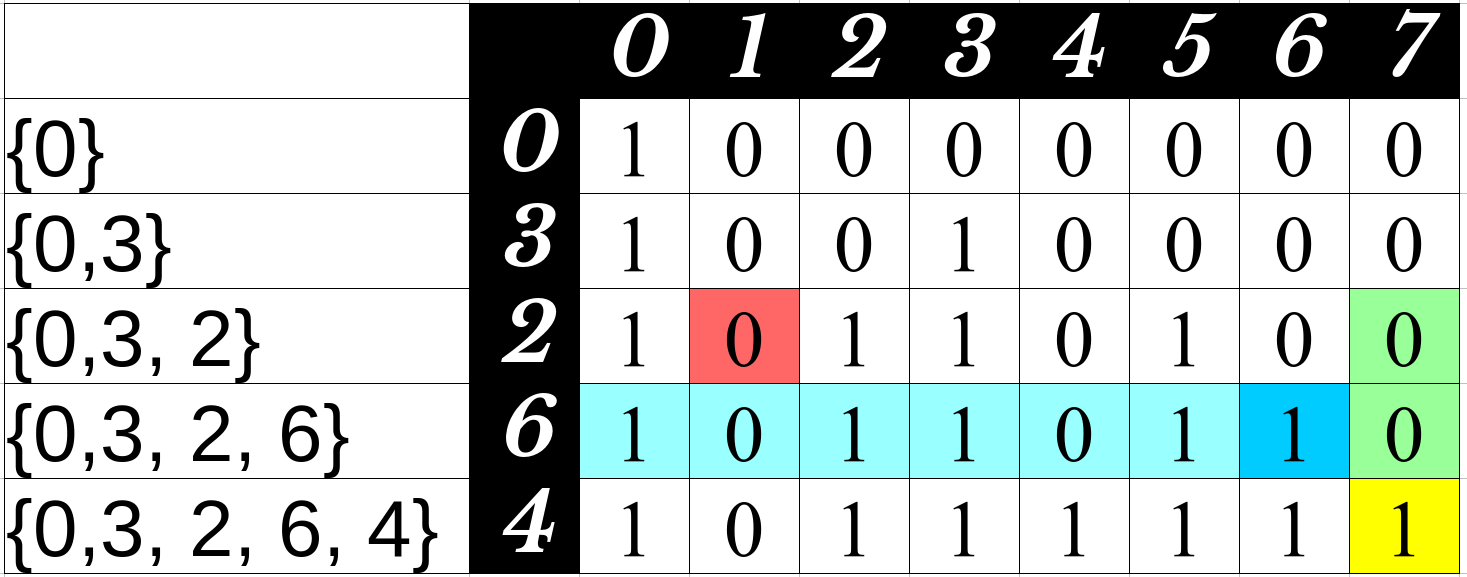
\includegraphics[width=10cm]{images/dyn1}
  \caption{Tableau dynamique dont les éléments indiquent l'existence (1) ou l'absence (0) de solution aux sous-problèmes $(T_i , y = 7)$ où $T_i$ est le sous-ensemble
  précisé en ligne $i$ indexée par la masse de l'objet et $y = 1, ...,7$. La case $(4,7)$ en jaune à 1 indique que le SSP possède au moins une solution.}
  \label{dyn1}
\end{figure}



\begin{figure}[htp]
  \centering
  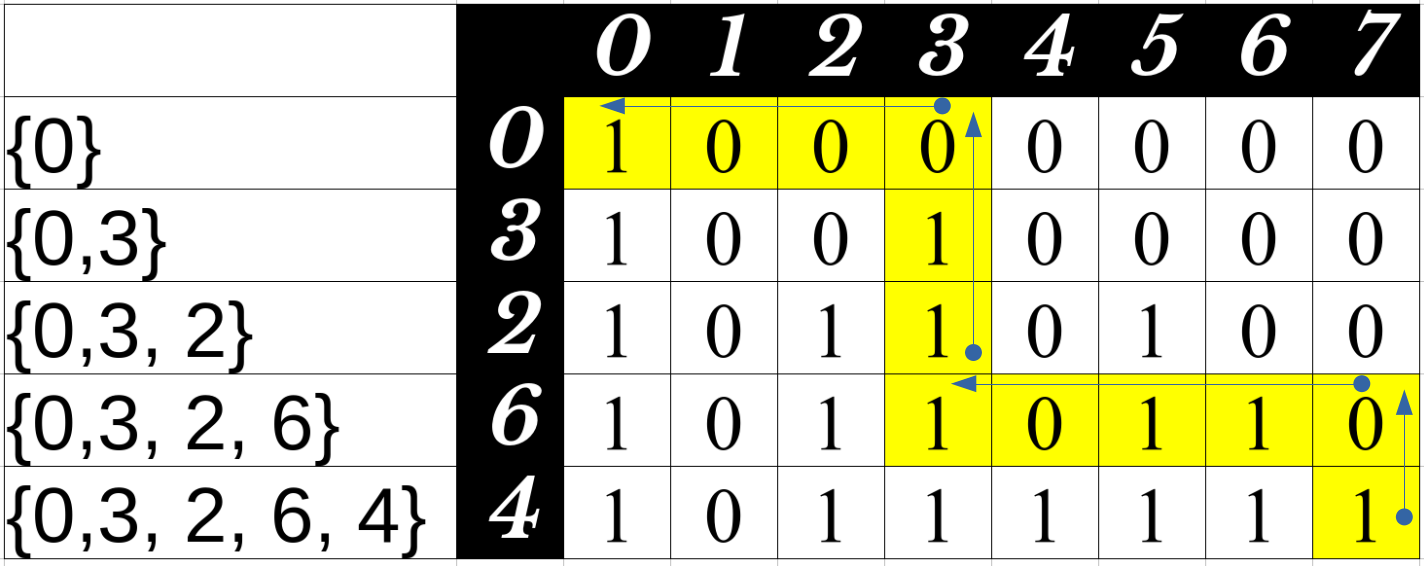
\includegraphics[width=10cm]{images/dyn2}
  \caption{Tableau dynamique : les lignes représentent les sous-ensembles, les colonnes les valeurs possibles du message y.}
  \label{dyn2}
\end{figure}

\paragraph{3\ieme{} phase - exploitation du tableau dynamique :} On détermine effectivement l'ensemble ordonné des objets à choisir pour obtenir le somme
désirée, c'est-à-dire le message en clair constitué de 0 et de 1. Dans cet exemple on doit trouver  $\{1, 0, 0, 1\}$
qui sélectionne les éléments 3 et 4, solutions du problème $(T = \{3, 2, 6, 4\}, y = 7)$. On part de la case $(4,7)$ calculée en dernier.
Si elle est surmontée d'un 0 cela signifie que le 4 fait partie de la solution. C'est le cas ici. On retire donc 4 à la somme $y = 7$, ce qui nous amène
à la case $(6,3)$ représentative du sous problème sachant que 4 a été sélectionné. La case du dessus $(2,3)$ est à 1, il n'a donc pas été nécessaire de sélectionner le 6.
idem pour le 2. On arrive à la case $(3,3)$, cette fois surmontée d'un 0. Le 3 est donc nécessaire à la solution du sous-problème. 
La sélection des objets s'arrête lorsqu'on arrive à la case $(0,0)$.

\subsubsection{Algorithme}

Dans l'algorithme ci-dessous, les indices font référence à notre implémentation où les indices de la clé vont de $0$ à $n-1$.

\begin{algorithm}[!h]
\caption{Résolution de $(T, y)$ par programmation dynamique}
\begin{algorithmic}[1]
\label{subset_algo}
\State $m \leftarrow$ matrice $(n+1) \times (y+1)$ initialisée à $false$
\For {$i = 0 \textbf{ to } n$ }
\State $m[i][0] \leftarrow true$
\EndFor
\For {$i = 1 \textbf{ to } n$}
\For {$j = 1 \textbf{ to } y$}
	\If {$j < t_{i-1}$}
		\State $m[i][j] \leftarrow m[i-1][j]$
	\Else
		\State $m[i][j] \leftarrow m[i-1][j] \textbf{ or } m[i-1][j-t_{i-1}]$
	\EndIf
\EndFor
\EndFor

\State $X \leftarrow$ tableau de taille $n$ initialisé à $0$
\State $i \leftarrow n$
\State $j \leftarrow y$
\While {$i > 0 \textbf{ and } j > 0$}
\If {$m[i-1][j] = false$}
\State $X[i-1] \leftarrow 1$
\State $j \leftarrow j - t_{i-1}$
\EndIf
\State $i \leftarrow i-1$
\EndWhile
\If {$j = 0$}
\State return $X$
\Else
\State return $NoSolution$
\EndIf
\end{algorithmic}
\end{algorithm}


\subsubsection{Complexité, résultats}

Les tests opérés sur un ordinateur classique sont conformes aux prévisions au vu de la complexité spatiale
de l'algorithme et de la croissance rapide des blocs en fonction de la taille de la clé : on tombe assez facilement à court de mémoire pour des tailles de clé de l'ordre de $n = 20$ (soit approximativement une occupation mémoire de 5 Go).

Les complexités spatiale et temporelle sont en $\mathcal{O}(n^2 \max T)$, le message $y$ étant, au pire, constitué de tous les éléments de $T$ et on a donc $y \leq n \times \max T$. D'après le paragraphe \ref{generation_cle} sur la génération des clés, $\max T$ est de l'ordre de $\mathcal{O}(2^n)$. Les complexités spatiale et temporelle de cet algorithme naïf sont donc vaguement en $\mathcal{O}(2^n n^2)$.

On comprend ainsi que cette méthode de cryptanalyse est très limitée, même sur une machine disposant d'une grande quantité de mémoire vive. Mettre en place une telle méthode demanderait également des optimisations que nous n'avons pas faites : les allocations de mémoire étant coûteuses, il faudrait si possible éviter de réallouer une telle matrice à chaque nouveau bloc, bien qu'elle dépende en partie de la valeur du bloc. De même, on pourrait imaginer une structure de données simulant une matrice de bits pour gagner un facteur en matière de complexité spatiale, bien que l'on se fasse vite rattraper par $n$…

\paragraph{} À plusieurs reprises, l'approche dynamique devait répondre sur l'existence d'une solution à un sous-problème du SSP. Dans la section suivante, nous mettrons pleinement à profit ces propriétés d'élagage en utilisant un arbre binaire de décision qui consiste à prendre ou à laisser un élément.


\subsection{Cryptanalyse récursive}
\label{rec}

\paragraph{} 
Soit à résoudre le SSP trivial précédent à savoir $(T = \{3, 2, 6, 4\}, y = 7)$. 
L'algorithme utilisé repose sur le parcours récursif d'un arbre étiqueté par des sommes partielles.
L'algorithme se décline en plusieurs phases :

\paragraph{1\iere{} phase - initialisation :} On commence par trier par ordre croissant l'ensemble $T$ et on résout donc le SPP trié $(T' = \{2, 3, 4, 6\}, y = 7)$
dont l'unique solution évidente correspond au message déchiffré $X' = \{x_0, x_1, x_2, x_3\} = \{0, 1, 1, 0\}$. Le tri croissant doit être effectué en conservant la permutation associée au tri qui nous permettra ensuite de retrouver $X = \{1, 0, 0, 1\}$ solution de $(T, y)$.

\paragraph{2\ieme{} phase - approche arborescente :} On trace un arbre binaire dont la racine porte une somme nulle comme en figure \ref{tree}. 
À la profondeur $p$, pour tout nœud de cet arbre, le fils gauche indiquera qu'on ne prend pas le $p$\ieme{} objet de l'ensemble $T'$ et au contraire, le fils droit indiquera qu'on sélectionne le $p$\ieme{} objet. L'étiquette d'un nœud correspond à la somme des objets sélectionnés jusque-là.

À la profondeur $p$, on observe donc les $2^{p}$ combinaisons possibles pour le sous-problème réduit aux $p$ premiers objets. Cette complexité temporelle exponentielle devient très vite impraticable. Il faut alors se demander s'il existe des critères qui permettraient de détecter les choix conduisant à une impasse de manière à pouvoir rebrousser chemin 
et « élaguer » notre arbre.


\paragraph{1\ier{} critère d'élagage :} On met en place deux critères d'élagage. Le premier est basé sur le fait que la somme courante, celle inscrite 
dans un nœud de notre arbre, additionnée des poids $t_i$ des éléments qui restent à choisir doit être supérieure à $y$. 
Sinon, on ne pourrait jamais atteindre l'objectif. Ce qu'on désigne couramment par « aller dans le mur » !
La 1\iere{} condition d'élagage $somme Courante + reliquat < y$ est donc :

\[\sum \limits_{i=0}^{k-1} x_{i}t_{i} + \sum \limits_{i=k}^{n-1} t_{i} < y\]

Par ailleurs, on pose 
\[S = \sum_{i=0}^{k-1} x_{i}t_{i}\] 
et 
\[r_k = \sum_{i=k}^{n-1} t_{i}\]

Pour faire le lien avec l'implémentation, la condition prend la forme : 
\[S + r_k < y\] dans le cas où on prend l'objet $k$, ou la forme :
\[S + r_k -t_k < y\] si on ne prend pas l'objet $k$ de masse $t_k$.

\paragraph{}
Exemple : si on ne prend pas les objets 2, 3 et 4, on a une somme courante nulle et un reliquat de $6 < y = 7$. 
Il est donc inutile de développer ce nœud. 

\paragraph{2\up{d} critère d'élagage :} Ce critère est basé sur le fait que si le terme $somme Courante + élémentSuivant$ est supérieur à m 
alors il n'est pas nécessaire de poursuivre dans cette voie car on dépasserait l'objectif en choisissant cet élément, l'ensemble $D'$ étant trié. On peut donc élaguer. On a donc la condition :
\[\sum_{i=0}^{k-1} x_{i}t_{i} + t_{k} > y\]

Ainsi sur la figure \ref{tree}, si on a une somme $S = 2$ à la profondeur 1 et qu'on s'interroge sur le fait de prendre ou non l'objet de poids $t_k = 3$ situé à la profondeur 2. 
Si on prend l'élément $t_{k+1}$ à la profondeur 3, on se retrouve avec une somme $S + t_k + t_{k+1} = 2 + 3 + 4 = 9 > 7$ 
donc on rebrousse chemin et on élague. l'arbre en abandonnant le choix qui consisterait à prendre l'élément 3. L'élagage revient donc à couper la branche 2-5. C'est le cœur de l'implémentation 
de l'algorithme rendu possible par le tri croissant de l'ensemble $D$. 


\paragraph{3\ieme{} phase - permutation inverse :} On permute la solution $X' = \{0, 1, 1, 0\}$ en utilisant la permutation associée au tri croissant de la phase 1.
On obtient ainsi le message décrypté $X = \{1, 0, 0, 1\}$ solution du SSP $(T = \{3, 2, 6, 4\}, y = 7)$.

\begin{figure}[htp]
  \centering
  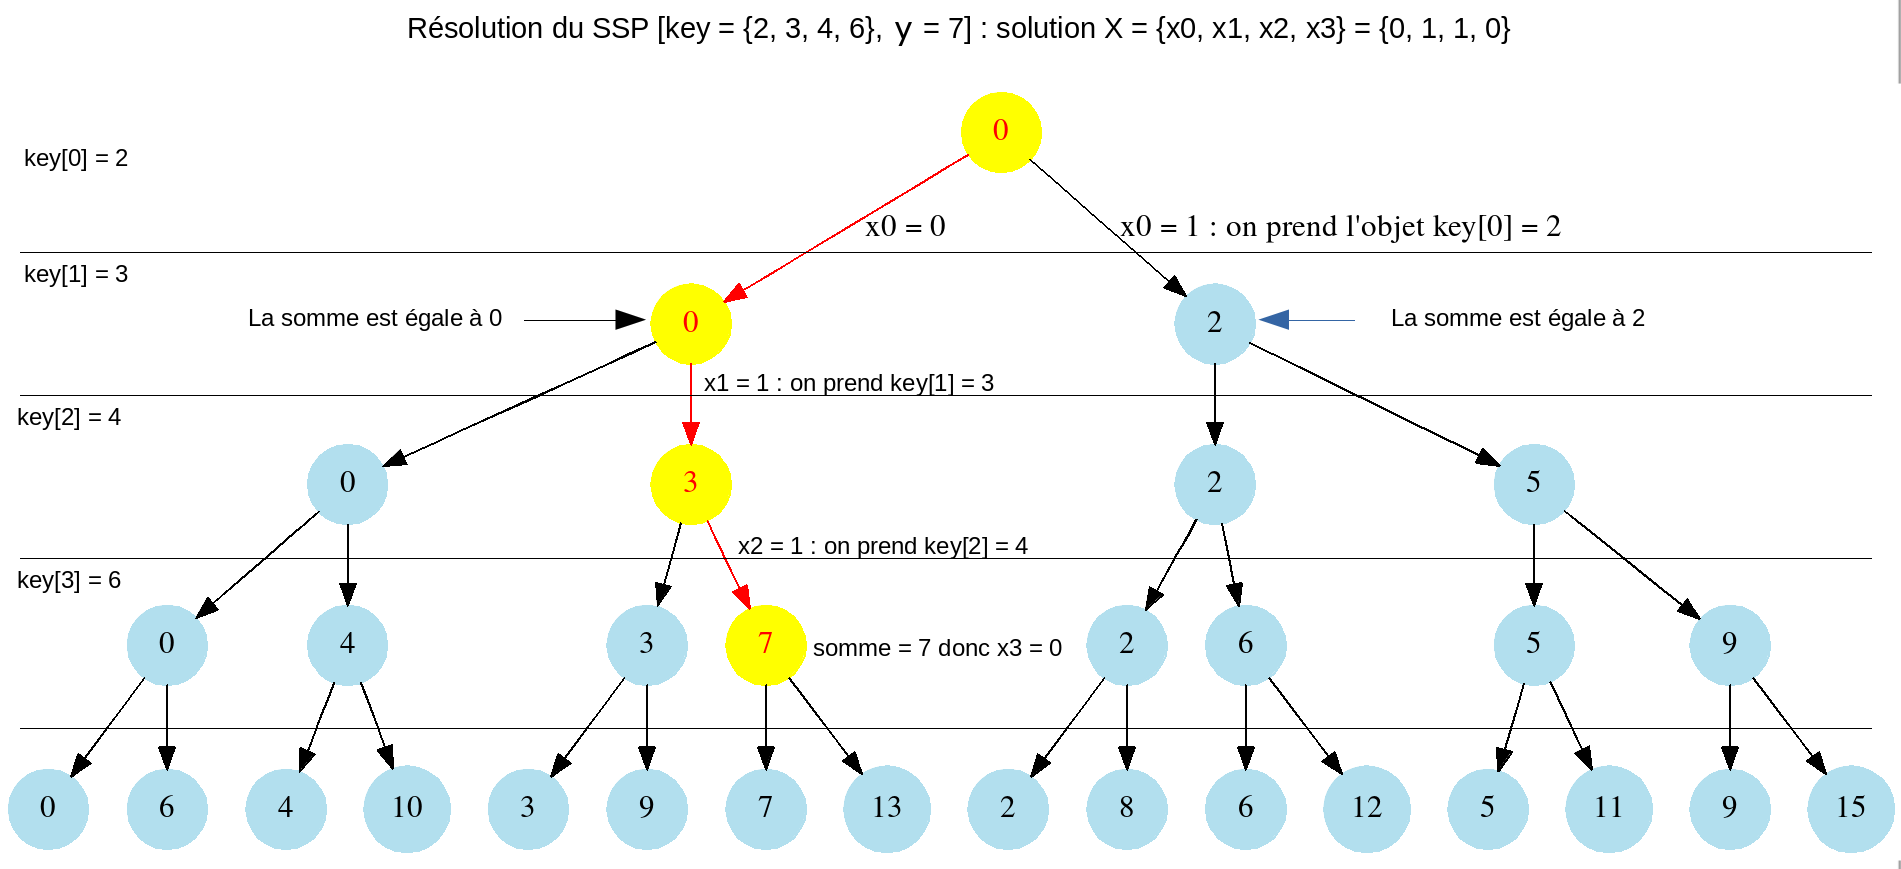
\includegraphics[width=16cm]{images/tree}
  \caption{Arbre de décision : le nœuds sont étiquetés par les sommes de sous-ensembles}
  \label{tree}
\end{figure}


\subsubsection{Complexité, résultats}

Les tests opérés sur un ordinateur classique montrent une capacité de cryptanalyse acceptable pour des tailles de clés
de l'ordre de 30. On rencontre un effet de seuil au-delà duquel le temps de calcul devient un véritable problème alors que l'occupation mémoire reste encore très limitée. Si ces élagages basiques permettent de guider la solution en évitant les parcours inutiles, ils n'enlèvent rien au caractère NP-complet du problème et la complexité en $\mathcal{O}(2^n)$ ne se fait oublier qu'un court instant. À ce stade où la mémoire n'est plus le problème principal car s'exprimant en $\mathcal{O}(n)$, on peut déjà
comprendre pourquoi les cryptosystèmes basés sur le principe du sac à dos ont été abandonnés. Ceci sans même parler des techniques 
par réduction de réseaux abordées dans la section suivante.